\documentclass[11pt]{article}
\usepackage[a4paper, margin=2cm]{geometry}
\usepackage{hyperref}
\usepackage{graphicx}
\usepackage{natbib}
\usepackage{float}
\usepackage[table,xcdraw]{xcolor}
\author{\bf \LARGE Research Proposal \\ \\ \bf Dito Eka Cahya (dc15772) FARSCOPE CDT 2015 \\\\ Supervised by : \\ Prof. Chris Melhuish, Dr. Praminda Caleb-Solly, Prof. Tony Pipe}
\date{}
\begin{document}
\title{\bf Towards The Development of Non-Verbal Multimodal Bidirectional Cognitive Architecture for Interactive Robot Assistant}
\maketitle
	\section{Aims \& Objectives}
		\subsection{Aims}
			\begin{itemize}
				\item[$\bullet$]The main aim of this research is to develop a basic model of cognitive architecture for a robot which is able to perceive and perform nonverbal multimodal natural interaction with human in real time. The design of proposed cognitive architecture is explained in ~\autoref{subsec:SystemBlockDiagram}.
				\item[$\bullet$]The second aim of this research is to implement and analyse the performance of the cognitive architecture in a robotic system which is situated in a “pick and handle” scenario. In this scenario, the robot is expected to detect human attention, recognize pointing gesture from human, infer and pick human required object, and handle the object to human in an appropriate way. The details of the scenario can be seen in ~\autoref{subsec:SystemFlowDiagram}.
			\end{itemize}
		\subsection{Objectives}
			\begin{itemize}
				\item[$\bullet$]Develop four perception subsystems to recognise nonverbal communication modes from human and to sense environment condition, which are pointing gesture, eye gaze, head pose, and object recognition subsystem.
				\item[$\bullet$]Develop multimodal perception inference engine to process and combine all perception inputs.
				\item[$\bullet$]Develop kinematics engine for robotic arm and head in order to enable nonverbal multimodal feedbacks from the robot such as pointing, picking, handling, gazing, and head movement.
				\item[$\bullet$]Develop cognitive engine to integrate perception, planning, and actuation subsystems.
				\item[$\bullet$]Develop learning algorithm to improve cognitive engine based on past task execution memory.
				\item[$\bullet$]Setup and integrate robotic system for implementing the cognitive architecture.
			\end{itemize}
	\section{Motivation}
		\begin{itemize}
			\item[$\bullet$]Recent studies conducted in~\cite{bemelmans2012socially},~\cite{national1999health}, and~\cite{Sharkey2012} have revealed that the number of elderly people in the population of the world has shown an increasing trend, due to increased life expectancy. On the other hand, the number of younger people is decreasing due to low birth rate. This will result in an unbalanced growth of caregivers and caretakers, putting pressure on the quality of the health care systems ~\cite{bemelmans2012socially}. Assisted living robots are one of the solution to solve this problem.
			\item[$\bullet$]In order to interact with human in most natural way, robot needs to have a multimodal communication capability, both verbal and nonverbal. (add reference)
			\item[$\bullet$]In a noisy environment, speech alone is not enough as communication mode, need to utilise other nonverbal communication modes such as gesture, eye gaze, head pose, etc to increase confidence of inferred human attention and intention. (add reference)
			\item[$\bullet$]In order to interact with human in most natural way, other than natural language capabilities, robot must also have cognitive architecture in order to solve general task. (add reference)
		\end{itemize}
	\section{Literature Review}
		\begin{itemize}
			\item[$\bullet$]Details of what has been described in Motivation section
			\item[$\bullet$]The design of theory of mind capabilities in interactive robotic agents is an important extension of social and cognitive capabilities in robots as it allows them to recognise the goals, intentions, desires, and belief of others. A robot can use its own theory of mind to improve the interaction with human users. ~\cite{scassellati2002theory}
			\item[$\bullet$]The term cognitive architecture, originally proposed in the field of computational cognitive modelling and artificial intelligence, refers to a broadly scoped, general purpose computational model that captures the essential structure and process of the mind. As such, it can be employed for wide ranging, multiple level, multiple domain modeling and simulation of behavior and cognitive phenomena, rather than focusing on separated, individual skills. ~\cite{sun2007importance}
				
		\end{itemize}
	\section{Basic Design}
		\subsection{System Block Diagram}
		\label{subsec:SystemBlockDiagram}
		~\autoref{fig:SystemBlockDiagram} shows general block diagram of cognitive architecture based on the generalisation of cognitive architecture design that has been done in~\cite{gordon2010neuromorphically},~\cite{forster2009robots}, and~\cite{vernon2011roadmap}. The proposed cognitive architecture will be based on those reference but developed toward generality, using the concept of developmental robotics~\cite{cangelosi2015developmental}. For the sake of simplicity, considering available time for Msc dissertation, I will focus on nonverbal inputs (pointing gesture,gaze,and head pose) and also object recognition for the cognitive architecture. 
			\begin{figure}[H]
				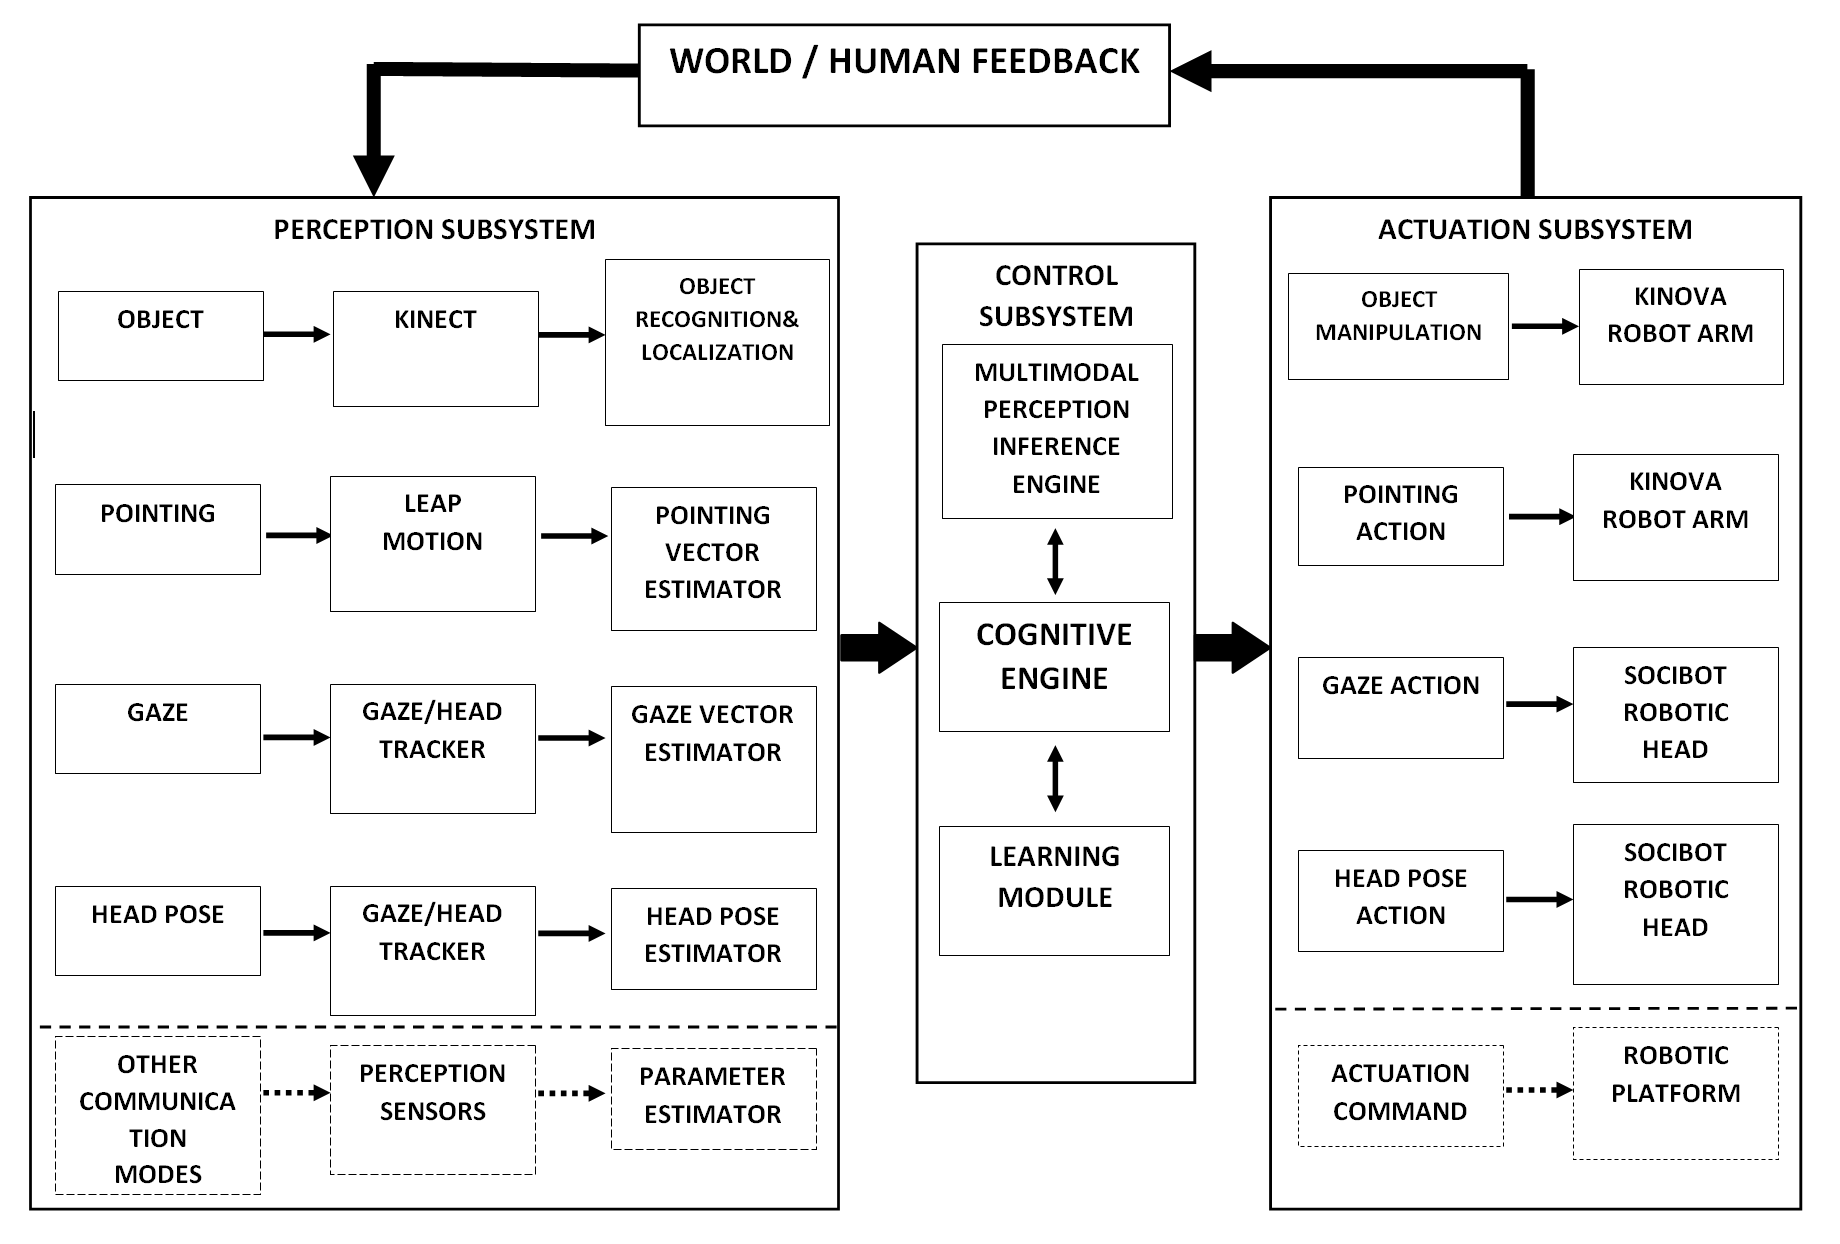
\includegraphics{BlockDiagram}
				\caption{General Cognitive Architecture Block Diagram \label{fig:SystemBlockDiagram}}
			\end{figure}
		\subsection{System Flow Diagram}
		\label{subsec:SystemFlowDiagram}
		In order to analyse the performance of cognitive architecture that will be developed, a "order, pick, and handle" scenario is proposed. ~\autoref{tab:Scenario} below shows the details of the scenario, along with involved communication modes on each step of the scenario.
		\begin{table}[H]
			\centering
			\caption{Scenario Description and Modalities Involved \label{tab:Scenario}}
			\begin{tabular}{ll|l|l|l|l|l|l|l|l|}
				\cline{3-10}
				&                                                                                                                                                                                                 & \multicolumn{4}{c|}{Perception Input}                                                                                                                                                               & \multicolumn{4}{c|}{Actuation Output}                                                                                                                                                               \\ \hline
				\multicolumn{1}{|l|}{S}  & Description                                                                                                                                                                                     & Gaze                     & \begin{tabular}[c]{@{}l@{}}Head \\ Pose\end{tabular} & \begin{tabular}[c]{@{}l@{}}Hand \\ Gesture\end{tabular} & \begin{tabular}[c]{@{}l@{}}Object\\ Recog.\end{tabular} & Gaze                     & \begin{tabular}[c]{@{}l@{}}Head \\ Pose\end{tabular} & \begin{tabular}[c]{@{}l@{}}Hand \\ Gesture\end{tabular} & \begin{tabular}[c]{@{}l@{}}Object\\ Manip.\end{tabular} \\ \hline
				\multicolumn{1}{|l|}{1}  & Wait human attention                                                                                                                                                                            & \cellcolor[HTML]{FE0000} & \cellcolor[HTML]{FE0000}                             &                                                         &                                                         &                          &                                                      &                                                         &                                                         \\ \hline
				\multicolumn{1}{|l|}{2}  & Look into human eyes                                                                                                                                                                            &                          &                                                      &                                                         &                                                         & \cellcolor[HTML]{FE0000} & \cellcolor[HTML]{FE0000}                             &                                                         &                                                         \\ \hline
				\multicolumn{1}{|l|}{3}  & Wait pointing gesture                                                                                                                                                                           & \cellcolor[HTML]{FE0000} & \cellcolor[HTML]{FE0000}                             & \cellcolor[HTML]{FE0000}                                &                                                         &                          &                                                      &                                                         &                                                         \\ \hline
				\multicolumn{1}{|l|}{4}  & \begin{tabular}[c]{@{}l@{}}Look at the direction\\ of pointing gesture\end{tabular}                                                                                                             &                          &                                                      &                                                         &                                                         & \cellcolor[HTML]{FE0000} & \cellcolor[HTML]{FE0000}                             &                                                         &                                                         \\ \hline
				\multicolumn{1}{|l|}{5}  & Infer required object                                                                                                                                                                           &                          &                                                      &                                                         & \cellcolor[HTML]{FE0000}                                &                          &                                                      &                                                         &                                                         \\ \hline
				\multicolumn{1}{|l|}{6}  & \begin{tabular}[c]{@{}l@{}}Point to inferred \\ object\end{tabular}                                                                                                                             &                          &                                                      &                                                         &                                                         &                          &                                                      & \cellcolor[HTML]{FE0000}                                &                                                         \\ \hline
				\multicolumn{1}{|l|}{7}  & Look into human eyes                                                                                                                                                                            & \cellcolor[HTML]{FE0000} & \cellcolor[HTML]{FE0000}                             &                                                         &                                                         & \cellcolor[HTML]{FE0000} & \cellcolor[HTML]{FE0000}                             &                                                         &                                                         \\ \hline
				\multicolumn{1}{|l|}{8}  & \begin{tabular}[c]{@{}l@{}}Wait for human\\ confirmation. If nod,\\ continue to step 9,\\ if shake, return to\\ step 3, if timeout or\\ losing attention, \\ return to step 1.\end{tabular}     & \cellcolor[HTML]{FE0000} & \cellcolor[HTML]{FE0000}                             &                                                         &                                                         &                          &                                                      &                                                         &                                                         \\ \hline
				\multicolumn{1}{|l|}{9}  & \begin{tabular}[c]{@{}l@{}}Look to the object\\ and pick object\end{tabular}                                                                                                                    &                          &                                                      &                                                         & \cellcolor[HTML]{FE0000}                                & \cellcolor[HTML]{FE0000} & \cellcolor[HTML]{FE0000}                             &                                                         & \cellcolor[HTML]{FE0000}                                \\ \hline
				\multicolumn{1}{|l|}{10} & \begin{tabular}[c]{@{}l@{}}Bring object toward\\ the direction of human\end{tabular}                                                                                                            &                          &                                                      &                                                         &                                                         &                          &                                                      &                                                         & \cellcolor[HTML]{FE0000}                                \\ \hline
				\multicolumn{1}{|l|}{11} & Look into human eyes                                                                                                                                                                            & \cellcolor[HTML]{FE0000} & \cellcolor[HTML]{FE0000}                             &                                                         &                                                         & \cellcolor[HTML]{FE0000} & \cellcolor[HTML]{FE0000}                             &                                                         &                                                         \\ \hline
				\multicolumn{1}{|l|}{12} & \begin{tabular}[c]{@{}l@{}}Wait for open palm\\ gesture (human hand\\ reaching toward \\ object). If detected, go\\ to step 14, if timeout\\ or losing attention go \\ to step 13.\end{tabular} & \cellcolor[HTML]{FE0000} & \cellcolor[HTML]{FE0000}                             & \cellcolor[HTML]{FE0000}                                &                                                         &                          &                                                      &                                                         &                                                         \\ \hline
				\multicolumn{1}{|l|}{13} & \begin{tabular}[c]{@{}l@{}}Look to object and\\ put object on that\\ location\end{tabular}                                                                                                      &                          &                                                      &                                                         & \cellcolor[HTML]{FE0000}                                & \cellcolor[HTML]{FE0000} & \cellcolor[HTML]{FE0000}                             &                                                         & \cellcolor[HTML]{FE0000}                                \\ \hline
				\multicolumn{1}{|l|}{14} & \begin{tabular}[c]{@{}l@{}}Look to object and\\ bring object closer\\ until on top of \\ the hand\end{tabular}                                                                                  &                          &                                                      &                                                         & \cellcolor[HTML]{FE0000}                                & \cellcolor[HTML]{FE0000} & \cellcolor[HTML]{FE0000}                             &                                                         & \cellcolor[HTML]{FE0000}                                \\ \hline
				\multicolumn{1}{|l|}{15} & Look into human eyes                                                                                                                                                                            & \cellcolor[HTML]{FE0000} & \cellcolor[HTML]{FE0000}                             &                                                         &                                                         & \cellcolor[HTML]{FE0000} & \cellcolor[HTML]{FE0000}                             &                                                         &                                                         \\ \hline
				\multicolumn{1}{|l|}{16} & \begin{tabular}[c]{@{}l@{}}Wait for human\\ confirmation. If nod,\\ continue to step 17,\\ if hand is withdrawn\\ and timeout, go to\\ step 13\end{tabular}                                     & \cellcolor[HTML]{FE0000} & \cellcolor[HTML]{FE0000}                             & \cellcolor[HTML]{FE0000}                                &                                                         &                          &                                                      &                                                         &                                                         \\ \hline
				\multicolumn{1}{|l|}{17} & \begin{tabular}[c]{@{}l@{}}Look to the object,\\ release the object,\\ return to step 1\end{tabular}                                                                                            &                          &                                                      &                                                         & \cellcolor[HTML]{FE0000}                                & \cellcolor[HTML]{FE0000} & \cellcolor[HTML]{FE0000}                             &                                                         & \cellcolor[HTML]{FE0000}                                \\ \hline
			\end{tabular}
		\end{table}
	\section{Risk Register}
		\begin{table}[H]
			\centering
			\caption{Risk register ranking}
			\label{my-label}
			\begin{tabular}{|l|l|l|l|l|}
				\hline
				\textbf{Risk}                                                                                                        & \textbf{Mitigation}                                                                                                                                                                                                                                                       & \textbf{\begin{tabular}[c]{@{}l@{}}Like\\ lihood\end{tabular}} & \textbf{\begin{tabular}[c]{@{}l@{}}Im\\ pact\end{tabular}} & \textbf{Score} \\ \hline
				\begin{tabular}[c]{@{}l@{}}Implementation failure of \\ the proposed method in one \\ or more subsystem\end{tabular} & \begin{tabular}[c]{@{}l@{}}Build and test subsystems as early as \\ possible, so that the methods can be changed \\ if they fail. Plan to implement more than \\ one method for each subsystem\end{tabular}                                                               & 3                                                              & 2                                                          & 6              \\ \hline
				\begin{tabular}[c]{@{}l@{}}Scenario is too complex for \\ the robot to be achieved\end{tabular}                      & \begin{tabular}[c]{@{}l@{}}Finish the development stage as soon as \\ possible so that we can improve the system if \\ it cannot achieve desired scenario. If this \\ option fails, simplify the scenario, without \\ sacrificing the purpose of experiment.\end{tabular} & 3                                                              & 2                                                          & 6              \\ \hline
				\begin{tabular}[c]{@{}l@{}}Failure of perception sensors \\ that are going to be used for \\ experiment\end{tabular} & \begin{tabular}[c]{@{}l@{}}Order more than one set of perception sensor\\ for each mode of nonverbal communication\end{tabular}                                                                                                                                           & 2                                                              & 3                                                          & 6              \\ \hline
				\begin{tabular}[c]{@{}l@{}}Late arrival of ordered \\ perception sensors\end{tabular}                                & \begin{tabular}[c]{@{}l@{}}Order the sensors as soon as possible and \\ borrow the sensors from other researchers \\ as a backup plan \\ (the sensors are widely used at BRL)\end{tabular}                                                                                & 2                                                              & 2                                                          & 4              \\ \hline
				\begin{tabular}[c]{@{}l@{}}Failure of robotic platform \\ that is going to be used for \\ experiment\end{tabular}    & \begin{tabular}[c]{@{}l@{}}Use robotic platform that is available more\\ than one set in BRL. If not possible, use \\ robotic platform that have similar type and \\ features with the primary one as a backup\end{tabular}                                               & 1                                                              & 4                                                          & 4              \\ \hline
			\end{tabular}
		\end{table}
	\section{Time line}
	The table below shows proposed project timeline. The project is started from week 2 of March and will be finished on week 2 of September, so the project will take 25 weeks to finish. 
	\begin{table}[H]
		\centering
		\caption{Project Timeline}
		\label{timeline_table}
		\begin{tabular}{lp{0.1cm}p{0.1cm}p{0.1cm}p{0.1cm}p{0.1cm}p{0.1cm}p{0.1cm}p{0.1cm}p{0.1cm}p{0.1cm}p{0.1cm}p{0.1cm}p{0.1cm}p{0.1cm}p{0.1cm}p{0.1cm}p{0.1cm}p{0.1cm}p{0.1cm}p{0.1cm}p{0.1cm}p{0.1cm}p{0.1cm}p{0.1cm}p{0.1cm}p{0.1cm}} \hline
			&                                                                      &                                               &                                               &                                               &                                               &                                               &                                               &                                               &                                               &                                               &                                               & W                                             & E                                             & E                                             & K                                             & S                                             &                                               &                                               &                                               &                                               &                                               &                                               &                                               &                                               &                                                                                              \\ \hline
			\multicolumn{1}{|l|}{Activity}                                                                                             &  \multicolumn{1}{l|}{\tiny 1}                        & \multicolumn{1}{l|}{\tiny 2}                        & \multicolumn{1}{l|}{\tiny 3}                        & \multicolumn{1}{l|}{\tiny 4}                        & \multicolumn{1}{l|}{\tiny 5}                        & \multicolumn{1}{l|}{\tiny 6}                        & \multicolumn{1}{l|}{\tiny 7}                        & \multicolumn{1}{l|}{\tiny 8}                        & \multicolumn{1}{l|}{\tiny 9}                       & \multicolumn{1}{l|}{\tiny 10}                       & \multicolumn{1}{l|}{\tiny 11}                       & \multicolumn{1}{l|}{\tiny 12}                       & \multicolumn{1}{l|}{\tiny 13}                       & \multicolumn{1}{l|}{\tiny 14}                       & \multicolumn{1}{l|}{\tiny 15}                       & \multicolumn{1}{l|}{\tiny 16}                       & \multicolumn{1}{l|}{\tiny 17}                       & \multicolumn{1}{l|}{\tiny 18}                       & \multicolumn{1}{l|}{\tiny 19}                       & \multicolumn{1}{l|}{\tiny 20}                       & \multicolumn{1}{l|}{\tiny 21}                       & \multicolumn{1}{l|}{\tiny 22}                       & \multicolumn{1}{l|}{\tiny 23}                       & \multicolumn{1}{l|}{\tiny 24}                       & \multicolumn{1}{l|}{\tiny 25}                       \\ \hline
			\multicolumn{1}{|l|}{\begin{tabular}[c]{@{}l@{}} \tiny Project \\ \tiny KickOff\end{tabular}}                                                                                      & \multicolumn{1}{l|}{}                         & \multicolumn{1}{l|}{}                         & \multicolumn{1}{l|}{}                         & \multicolumn{1}{l|}{}                         & \multicolumn{1}{l|}{}                         & \multicolumn{1}{l|}{}                         & \multicolumn{1}{l|}{}                         & \multicolumn{1}{l|}{}                         & \multicolumn{1}{l|}{}                         & \multicolumn{1}{l|}{}                         & \multicolumn{1}{l|}{}                         & \multicolumn{1}{l|}{}                         & \multicolumn{1}{l|}{}                         & \multicolumn{1}{l|}{}                         & \multicolumn{1}{l|}{}                         & \multicolumn{1}{l|}{}                         & \multicolumn{1}{l|}{}                         & \multicolumn{1}{l|}{}                         & \multicolumn{1}{l|}{}                         & \multicolumn{1}{l|}{}                         & \multicolumn{1}{l|}{}                         & \multicolumn{1}{l|}{}                         & \multicolumn{1}{l|}{}                         & \multicolumn{1}{l|}{}                         & \multicolumn{1}{l|}{}                         \\ \hline
			\multicolumn{1}{|l|}{\begin{tabular}[c]{@{}l@{}} \tiny Literature \\ \tiny Revicw\end{tabular}}                                                                                                           & \multicolumn{1}{l|}{\cellcolor[HTML]{FE0000}} & \multicolumn{1}{l|}{\cellcolor[HTML]{FE0000}} & \multicolumn{1}{l|}{\cellcolor[HTML]{FE0000}} & \multicolumn{1}{l|}{\cellcolor[HTML]{FE0000}} & \multicolumn{1}{l|}{\cellcolor[HTML]{FE0000}} & \multicolumn{1}{l|}{\cellcolor[HTML]{FE0000}} & \multicolumn{1}{l|}{\cellcolor[HTML]{FE0000}} & \multicolumn{1}{l|}{\cellcolor[HTML]{FE0000}} & \multicolumn{1}{l|}{\cellcolor[HTML]{FE0000}} & \multicolumn{1}{l|}{\cellcolor[HTML]{FE0000}} & \multicolumn{1}{l|}{\cellcolor[HTML]{FE0000}} & \multicolumn{1}{l|}{\cellcolor[HTML]{FE0000}} & \multicolumn{1}{l|}{\cellcolor[HTML]{FE0000}} & \multicolumn{1}{l|}{\cellcolor[HTML]{FE0000}} & \multicolumn{1}{l|}{\cellcolor[HTML]{FE0000}} & \multicolumn{1}{l|}{}                         & \multicolumn{1}{l|}{}                         & \multicolumn{1}{l|}{}                         & \multicolumn{1}{l|}{}                         & \multicolumn{1}{l|}{}                         & \multicolumn{1}{l|}{}                         & \multicolumn{1}{l|}{}                         & \multicolumn{1}{l|}{}                         & \multicolumn{1}{l|}{}                         & \multicolumn{1}{l|}{}                         \\ \hline
			\multicolumn{1}{|l|}{\begin{tabular}[c]{@{}l@{}} \tiny Project \\ \tiny Planning\\ \tiny Basic Design\end{tabular}}                                                     & \multicolumn{1}{l|}{\cellcolor[HTML]{FE0000}} & \multicolumn{1}{l|}{\cellcolor[HTML]{FE0000}} & \multicolumn{1}{l|}{\cellcolor[HTML]{FE0000}} & \multicolumn{1}{l|}{}                         & \multicolumn{1}{l|}{}                         & \multicolumn{1}{l|}{}                         & \multicolumn{1}{l|}{}                         & \multicolumn{1}{l|}{}                         & \multicolumn{1}{l|}{}                         & \multicolumn{1}{l|}{}                         & \multicolumn{1}{l|}{}                         & \multicolumn{1}{l|}{}                         & \multicolumn{1}{l|}{}                         & \multicolumn{1}{l|}{}                         & \multicolumn{1}{l|}{}                         & \multicolumn{1}{l|}{}                         & \multicolumn{1}{l|}{}                         & \multicolumn{1}{l|}{}                         & \multicolumn{1}{l|}{}                         & \multicolumn{1}{l|}{}                         & \multicolumn{1}{l|}{}                         & \multicolumn{1}{l|}{}                         & \multicolumn{1}{l|}{}                         & \multicolumn{1}{l|}{}                         & \multicolumn{1}{l|}{}                         \\ \hline
			\multicolumn{1}{|l|}{\begin{tabular}[c]{@{}l@{}}\tiny Develop and \\ \tiny Test \\ \tiny Perception\\ \tiny Subsystems,\\ \tiny Order Sensors.\end{tabular}}                     & \multicolumn{1}{l|}{}                         & \multicolumn{1}{l|}{}                         & \multicolumn{1}{l|}{}                         & \multicolumn{1}{l|}{\cellcolor[HTML]{FE0000}} & \multicolumn{1}{l|}{\cellcolor[HTML]{FE0000}} & \multicolumn{1}{l|}{\cellcolor[HTML]{FE0000}} & \multicolumn{1}{l|}{\cellcolor[HTML]{FE0000}} & \multicolumn{1}{l|}{\cellcolor[HTML]{FE0000}} & \multicolumn{1}{l|}{}                         & \multicolumn{1}{l|}{}                         & \multicolumn{1}{l|}{}                         & \multicolumn{1}{l|}{}                         & \multicolumn{1}{l|}{}                         & \multicolumn{1}{l|}{}                         & \multicolumn{1}{l|}{}                         & \multicolumn{1}{l|}{}                         & \multicolumn{1}{l|}{}                         & \multicolumn{1}{l|}{}                         & \multicolumn{1}{l|}{}                         & \multicolumn{1}{l|}{}                         & \multicolumn{1}{l|}{}                         & \multicolumn{1}{l|}{}                         & \multicolumn{1}{l|}{}                         & \multicolumn{1}{l|}{}                         & \multicolumn{1}{l|}{}                         \\ \hline
			\multicolumn{1}{|l|}{\begin{tabular}[c]{@{}l@{}}\tiny Develop and \\ \tiny Test Control \\ \tiny Subsystems\end{tabular}}                                            & \multicolumn{1}{l|}{}                         & \multicolumn{1}{l|}{}                         & \multicolumn{1}{l|}{}                         & \multicolumn{1}{l|}{}                         & \multicolumn{1}{l|}{}                         & \multicolumn{1}{l|}{}                         & \multicolumn{1}{l|}{}                         & \multicolumn{1}{l|}{}                         & \multicolumn{1}{l|}{\cellcolor[HTML]{FE0000}} & \multicolumn{1}{l|}{\cellcolor[HTML]{FE0000}} & \multicolumn{1}{l|}{\cellcolor[HTML]{FE0000}} & \multicolumn{1}{l|}{\cellcolor[HTML]{FE0000}} & \multicolumn{1}{l|}{\cellcolor[HTML]{FE0000}} & \multicolumn{1}{l|}{} & \multicolumn{1}{l|}{} & \multicolumn{1}{l|}{}                         & \multicolumn{1}{l|}{}                         & \multicolumn{1}{l|}{}                         & \multicolumn{1}{l|}{}                         & \multicolumn{1}{l|}{}                         & \multicolumn{1}{l|}{}                         & \multicolumn{1}{l|}{}                         & \multicolumn{1}{l|}{}                         & \multicolumn{1}{l|}{}                         & \multicolumn{1}{l|}{}                         \\ \hline
			\multicolumn{1}{|l|}{\begin{tabular}[c]{@{}l@{}}\tiny Develop and \\ \tiny Test Actuator\\ \tiny Subsystems\end{tabular}}                                            & \multicolumn{1}{l|}{}                         & \multicolumn{1}{l|}{}                         & \multicolumn{1}{l|}{}                         & \multicolumn{1}{l|}{}                         & \multicolumn{1}{l|}{}                         & \multicolumn{1}{l|}{}                         & \multicolumn{1}{l|}{}                         & \multicolumn{1}{l|}{}                         & \multicolumn{1}{l|}{}                         & \multicolumn{1}{l|}{}                         & \multicolumn{1}{l|}{}                         & \multicolumn{1}{l|}{}                         & \multicolumn{1}{l|}{}                         & \multicolumn{1}{l|}{\cellcolor[HTML]{FE0000}} & \multicolumn{1}{l|}{\cellcolor[HTML]{FE0000}} & \multicolumn{1}{l|}{} & \multicolumn{1}{l|}{} & \multicolumn{1}{l|}{}                         & \multicolumn{1}{l|}{}                         & \multicolumn{1}{l|}{}                         & \multicolumn{1}{l|}{}                         & \multicolumn{1}{l|}{}                         & \multicolumn{1}{l|}{}                         & \multicolumn{1}{l|}{}                         & \multicolumn{1}{l|}{}                         \\ \hline
			\multicolumn{1}{|l|}{\begin{tabular}[c]{@{}l@{}}\tiny System \\ \tiny Integration\end{tabular}}                                                                                                                             & \multicolumn{1}{l|}{}                         & \multicolumn{1}{l|}{}                         & \multicolumn{1}{l|}{}                         & \multicolumn{1}{l|}{}                         & \multicolumn{1}{l|}{}                         & \multicolumn{1}{l|}{}                         & \multicolumn{1}{l|}{}                         & \multicolumn{1}{l|}{}                         & \multicolumn{1}{l|}{}                         & \multicolumn{1}{l|}{}                         & \multicolumn{1}{l|}{}                         & \multicolumn{1}{l|}{}                         & \multicolumn{1}{l|}{}                         & \multicolumn{1}{l|}{}                         & \multicolumn{1}{l|}{}                         & \multicolumn{1}{l|}{\cellcolor[HTML]{FE0000}} & \multicolumn{1}{l|}{\cellcolor[HTML]{FE0000}} & \multicolumn{1}{l|}{}                         & \multicolumn{1}{l|}{}                         & \multicolumn{1}{l|}{}                         & \multicolumn{1}{l|}{}                         & \multicolumn{1}{l|}{}                         & \multicolumn{1}{l|}{}                         & \multicolumn{1}{l|}{}                         & \multicolumn{1}{l|}{}                         \\ \hline
			\multicolumn{1}{|l|}{\tiny Run Scenario}                                                                                                                                       & \multicolumn{1}{l|}{}                         & \multicolumn{1}{l|}{}                         & \multicolumn{1}{l|}{}                         & \multicolumn{1}{l|}{}                         & \multicolumn{1}{l|}{}                         & \multicolumn{1}{l|}{}                         & \multicolumn{1}{l|}{}                         & \multicolumn{1}{l|}{}                         & \multicolumn{1}{l|}{}                         & \multicolumn{1}{l|}{}                         & \multicolumn{1}{l|}{}                         & \multicolumn{1}{l|}{}                         & \multicolumn{1}{l|}{}                         & \multicolumn{1}{l|}{}                         & \multicolumn{1}{l|}{}                         & \multicolumn{1}{l|}{}                         & \multicolumn{1}{l|}{}                         & \multicolumn{1}{l|}{\cellcolor[HTML]{FE0000}} & \multicolumn{1}{l|}{\cellcolor[HTML]{FE0000}} & \multicolumn{1}{l|}{\cellcolor[HTML]{FE0000}} & \multicolumn{1}{l|}{\cellcolor[HTML]{FE0000}} & \multicolumn{1}{l|}{}                         & \multicolumn{1}{l|}{}                         & \multicolumn{1}{l|}{}                         & \multicolumn{1}{l|}{}                         \\ \hline
			\multicolumn{1}{|l|}{\tiny Write Up}                                                                                                                                           & \multicolumn{1}{l|}{}                         & \multicolumn{1}{l|}{}                         & \multicolumn{1}{l|}{}                         & \multicolumn{1}{l|}{}                         & \multicolumn{1}{l|}{}                         & \multicolumn{1}{l|}{}                         & \multicolumn{1}{l|}{}                         & \multicolumn{1}{l|}{}                         & \multicolumn{1}{l|}{}                         & \multicolumn{1}{l|}{}                         & \multicolumn{1}{l|}{}                         & \multicolumn{1}{l|}{}                         & \multicolumn{1}{l|}{}                         & \multicolumn{1}{l|}{}                         & \multicolumn{1}{l|}{}                         & \multicolumn{1}{l|}{}                         & \multicolumn{1}{l|}{}                         & \multicolumn{1}{l|}{}                         & \multicolumn{1}{l|}{}                         & \multicolumn{1}{l|}{}                         & \multicolumn{1}{l|}{}                         & \multicolumn{1}{l|}{\cellcolor[HTML]{FE0000}} & \multicolumn{1}{l|}{\cellcolor[HTML]{FE0000}} & \multicolumn{1}{l|}{\cellcolor[HTML]{FE0000}} & \multicolumn{1}{l|}{\cellcolor[HTML]{FE0000}} \\ \hline
		\end{tabular}
	\end{table}
	\section{References}
	\bibliography{ditoRef}
	\bibliographystyle{agsm}
\end{document}